\subsubsection{Group Permissions}

\paragraph{Extending Individual Access Control}

Group permissions extend the above system for individual permissions and require the use of smart contracts.

Whilst our application is intended to be fully decentralised, the key stakeholders for some applications (such as health care) may require access to the network to administrate. One example of this is the involvement of the GMC in validating doctor identities. If a doctor has not been registered, or has been struck off, they should not have any access to patient data (even if they claim to be a doctor). They should only have access should the GMC validate that they are in fact a valid doctor.

The idea of a group administrator, such as the GMC, conflicts with the idea of the data owner maintaining full access control and administration. However, should the data owner decide that the group should no longer have any access or wishes to change group permissions, they are able to do so.

To facilitate this, let's take a look at the architecture of a group's interactions with a particular identity's contract.

\begin{figure}[H]
  \centering
  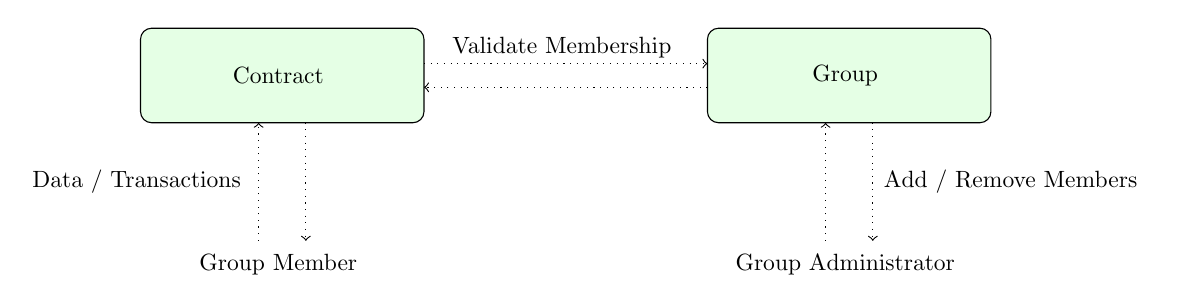
\begin{tikzpicture}[scale = 0.6, every node/.style={scale = 0.85}, every node/.append style={fill = white, rounded corners = 2pt, inner sep = 2pt, align = center}]

  \draw [rounded corners, fill=green!10] (-3, 1) rectangle (3, -1);
  \node [fill=green!10] at (0, 0) { Contract };

  \node at (-3, -2.25) { Data / Transactions };
  \draw [ -> , dotted] (-0.5, -3.5) -- (-0.5, -1);
  \draw [ -> , dotted] (0.5,  -1) -- (0.5,  -3.5);

  \node at (0, -4) { Group Member };

  \draw [rounded corners, fill=green!10] (9, 1) rectangle (15, -1);
  \node [fill=green!10] at (12, 0) { Group };

  \node at (15.5, -2.25) { Add / Remove Members };
  \draw [ -> , dotted] (11.5, -3.5) -- (11.5,    -1);
  \draw [ -> , dotted] (12.5,   -1) -- (12.5,  -3.5);

  \node at (12, -4) { Group Administrator };

  \node at (6, 0.6) { Validate Membership };
  \draw [ -> , dotted] (3,  0.25) -- (9,  0.25);
  \draw [ -> , dotted] (9, -0.25) -- (3, -0.25);

  \end{tikzpicture} \\
  \caption{
  	How a group interacts with an identity's data
  }
  \label{fig:archi_group_interactions}
\end{figure}


An identity claiming to be a member of a group will always interact with the storage contract it is trying to retrieve from or add data to. A group itself will never be able to directly affect or transact with a storage contract such that no malicious attacker would be able to pseudo-anonymously act as the group.

When the identity tries to access a path, their identity is cross-checked with the group they claim to be a member of. Should this group validate the identity as a member, and assuming the group has the necessary permissions that are required to action the identity's transaction, the transaction will be successful.

\paragraph{Group Key Sharing}

Whilst the process of writing data is similar to an individual (other than the membership validation above), the process of reading data differs hugely for groups.

If we were to extend the process of reading as an individual to a group, the result would be a process similar to this:

\begin{figure}[H]
  \centering
  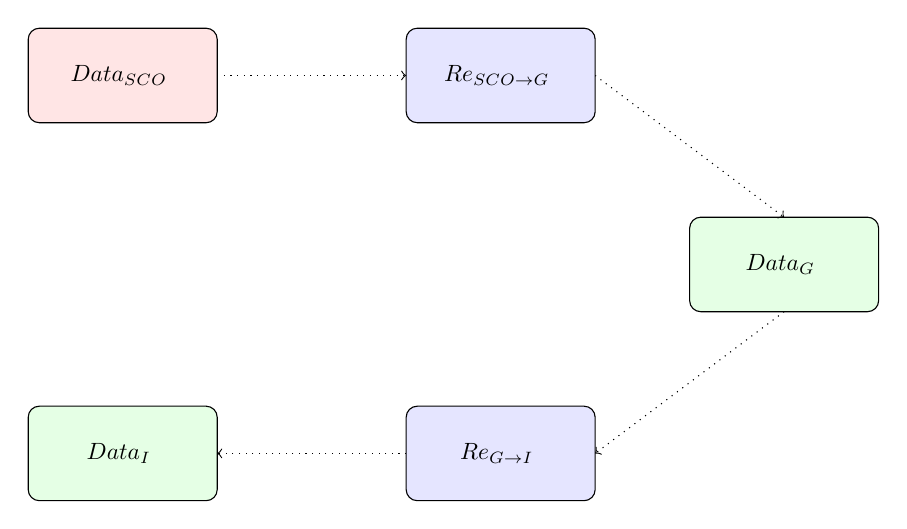
\begin{tikzpicture}[scale = 0.6, every node/.style={scale = 0.85}, every node/.append style={fill = white, rounded corners = 2pt, inner sep = 2pt, align = center}]

  \draw [rounded corners, fill=green!10] (-10, -7) rectangle (-6, -9);
  \node [fill=green!10] at (-8, -8) { $\text{Data}_{\text{I}}$ };

  \draw [ -> , dotted] (-2, -8) -- (-6, -8);

  \draw [rounded corners, fill=blue!10] (-2, -7) rectangle (2, -9);
  \node [fill=blue!10] at (0, -8) { $\text{Re}_{\text{G} \rightarrow \text{I}}$ };

  \draw [ -> , dotted] (6, -5) -- (2, -8);

  \draw [rounded corners, fill=green!10] (4, -3) rectangle (8, -5);
  \node [fill=green!10] at (6, -4) { $\text{Data}_{\text{G}}$ };

  \draw [ -> , dotted] (2, 0) -- (6, -3);

  \draw [rounded corners, fill=blue!10] (-2, 1) rectangle (2, -1);
  \node [fill=blue!10] at (0, 0) { $\text{Re}_{\text{SCO} \rightarrow \text{G}}$ };

  \draw [ -> , dotted] (-6, 0) -- (-2, 0);

  \draw [rounded corners, fill=red!10] (-6, 1) rectangle (-10, -1);
  \node [fill=red!10] at (-8, 0) { $\text{Data}_{\text{SCO}}$ };

  \end{tikzpicture} \\
  \caption{
  	Group Read Re-encryption (theoretical)
  }{
    The theoretical process of re-encrypting from a storage contract owner to a group, then re-encrypting again from the group to an individual (member of the group).
  }
  \label{fig:encryption_group_read_theoretical}
\end{figure}

